\chapter{Top-down Constraints on Atmospheric Mercury Emissions from ASGM Activities}\label{Chapter3}
To measure the effectiveness of mitigation and elimination strategies for reducing Hg pollution from ASGM, Hg emissions estimates will be compared to baseline estimates per Article 22 of the MC. The ASGM industry is often unregulated, with little government oversight and a limited amount of reliable data\cite{oneill_estimating_2017}.  Therefore, measurement of Hg use in the ASGM sector is difficult due to its complexity and largely informal nature.  Typically, finding reasonable estimates of ASGM Hg use, gold production, and staff requires extensive site visits, multiple interviews, observations, and measurements at ASGM sites\cite{oneill_estimating_2017}.
\begin{flushleft}
In this chapter, I apply a top-down approach at a regional scale to estimate ASGM Hg emissions (emission inversion) from Peru. As of now, there has been no scientific study using Hg atmospheric monitoring data and atmospheric models to provide top-down constraints for ASGM emissions. Section \ref{c3_methods} describes the overall methodology. I combine ground-based observations of atmospheric Hg from the case study region\cite{koenig_seasonal_2021}, a national inventory for Peru\cite{artisanal_gold_council_reporte_2017} and simulations with the GEOS-Chem global CTM. Reference (also known as a priori) emissions are from the GMA 2018\cite{united_nations_environment_programme_technical_2019,steenhuisen_development_2019}. The Markov Chain Monte Carlo is the inversion method used (Sect. \ref{c3_mcmc}) to obtain the optimized (a posteriori) emissions, considering uncertainties associated with reference and ground-based observations. Section \ref{c3_results} presents results and discussion. Comparisons of observations and model outputs are given in Sect. \ref{c3_obs_v_modifications}. The optimized emissions from 5 regions in Peru are shown in Sect.\ref{c3_mcmc_estimates}. Finally, I discuss the implications of the inversion results for providing baseline estimates of ASGM Hg emissions and summarize my conclusions (Sect. \ref{c3_conclusion}).

\end{flushleft}
\section{Background}
\begin{flushleft}


 Numerous prior studies have quantified anthropogenic Hg sources, including ASGM Hg emissions using different methodologies. Bottom-up estimates leverage collected data on underlying activities and emission factors to estimate regional and global totals. For instance, the bottom-up global inventory in the GMA 2018 estimated ASGM Hg emissions to be 838 Mg with an uncertainty range of 675-1000 Mg for 2015 \cite{united_nations_environment_programme_technical_2019,steenhuisen_development_2019}. Moreover, Streets et al. (2019) tested six different proxies for scaling emissions to other years and used an average value to scale the inventory of emissions to the year 2015, thus estimating that ASGM was the largest source and responsible for 775 Mg of emissions\cite{streets_global_2019}. Muntean et al. (2014) also used a bottom-up technique in which they found that poverty in gold ore-rich countries (as measured by the GINI index \cite{sadefo_kamdem_nice_2012}, where available) was correlated with data on ASGM production activity. The poverty-based approach they used estimated that ASGM was responsible for 728.27 Mg emissions in 2010, equivalent to 41.1\% of the global Hg emissions\cite{muntean_evaluating_2018}. Such inventories are essential and a critical input to model Hg using CTMs such as \gc. 
 \end{flushleft}
 
 \begin{flushleft}
 However, the different assumptions on the activity data and emission factors induce significant uncertainty in the emission inventories. Furthermore, the bottom-up approach has biases due to its reliance on officially reported emission data, which may cause regional and national differences in accuracy. Countries identify and quantify Hg sources released within their borders through national baseline Hg-use estimates as per O'neill and Telmer\cite{oneill_estimating_2017}. Under Article 7 of the MC and Annex C, countries must include in their NAPs baseline estimates of the quantities of mercury used in ASGM within their territory\cite{united_nations_environment_programme_estimating_2017}.  
 \end{flushleft}
 



\begin{flushleft}
In contrast to bottom-up approaches, top-down emission estimation approaches combine atmospheric transport and chemistry models with atmospheric concentration measurements to quantify emissions. Even though the atmospheric chemistry literature has various top-down method applications, no study explicitly constrains ASGM Hg emissions. For instance, Bousquet et al., 1999 applied top-down methods to infer surface fluxes of atmospheric CO\textsubscript{2} from observed concentrations\cite{bousquet_inverse_1999}. Furthermore, Kopacz et al., 2009, employed top-down techniques to quantify source contributions to ozone pollution at two adjacent sites on the U.S. west coast in the spring of 2006\cite{kopacz_global_2010}. They used  \gc as a common intercomparison platform to show global consistency between the satellite data sets and the in situ data. This underscores the role models such as GEOS-chem have as integration platforms for differently sourced data to generate unified insights. Likewise, Hg emissions have been constrained using top-down methods in Song et al., 2015 where a top-down approach at a global scale is applied to quantitatively estimate present-day Hg emission sources and critical parameters in GEOS-Chem to better constrain the global biogeochemical cycle of Hg\cite{song_top-down_2015}. Moreover, Denzler et al., 2017 used a top-down approach to quantify Hg emissions on a European scale based on the atmospheric Hg measurements conducted at the remote high-altitude monitoring station, Jungfraujoch, Switzerland\cite{denzler_inversion_2017}. 
\end{flushleft}


\section{Methods}\label{c3_methods}
\begin{flushleft}
    Chapter 2 of this thesis discusses the differences between the \gc model predictions of Hg at various monitoring stations and in Latin America. In one hypothesis, the difference between the model and the observations was attributed to how the emissions were parameterized in \gc. Generally, the input emissions in \gc are determined by the Hg inventory used; hence, I first evaluated the Hg inventory used in the simulations in Chapter 2 (GMA 2018, also called AMAP/UNEP 2015 inventory) against other global inventories. Next, the inventory was compared to a national inventory for Peru developed by the Artisanal Gold Council in preparation for Peru's NAP \cite{agc_reporte_2017}. Once the differences between the GMA 2018 inventory\cite{steenhuisen_development_2019} and the Peruvian national inventory were analyzed \cite{agc_reporte_2017}, the global inventory was re-gridded to the GEOS-Chem grid, and the emissions from grid boxes corresponding to different departments in Peru were scaled. The scaled inventories were used to create the simulations described in Table \ref{tab:all_geos_chem_simulations}. These simulations were used to investigate the sensitivity of the Hg concentration at distant locations to the changes in emissions from the grid boxes in the case study region. The simulated \hgc in the atmosphere was compared to the observed TGM concentration in the atmosphere to determine the sensitivity of the \hgc to the changes in emissions from individual grid boxes and multiple grid boxes. 
\end{flushleft}

\subsection{Mercury Emission Inventories}\label{c3_Mercury Emission Inventories}
\begin{flushleft}


Globally gridded emissions inventories such as those shown in Figure \ref{fig:Hg_inventories} are a critical input to CTMs such as \gc. Figure \ref{fig:Hg_inventories} shows the distribution of Peruvian anthropogenic Hg emission estimates by different global inventories \cite{united_nations_environment_programme_technical_2019,steenhuisen_development_2019,streets_global_2019,muntean_evaluating_2018}.  The GMA 2018 ASGM Hg emissions estimates for 2015 are shown in Figure \ref{fig:Hg_inventories}, (a). The ASGM Hg emissions in the GMA 2018 inventory were distributed by assigning emission estimates to geo-located point sources, using reported emissions information where available, and otherwise assigning a modeled emission to the point. Emissions that could not be assigned to point sources were distributed using sector-specific proxies \cite{steenhuisen_development_2019}. The proxies for ASGM Hg emissions in Peru were the locations of legal mining concessions and the global alluvial gold map \href{(https://data.globalforestwatch.org/search?collection=Dataset&q=mining)}{data set}. This inventory estimated that ASGM was responsible for about 110 tonnes of annual emissions in Peru. Moreover, the GMA 2018 inventory was used in all the GEOS-Chem simulations conducted in this study. This inventory was used because it was more representative of the ASGM emissions than the other two inventories, as the total Hg emissions are compatible with bottom-up baseline ASGM Hg emissions. Figure \ref{fig:Hg_inventories},(b) shows how anthropogenic Hg emissions were distributed in the EDGAR ASGM Hg emissions inventory\cite{muntean_evaluating_2018}. This global mercury emissions inventory includes emissions from all key mercury emitting sources, and Peru's total Hg emissions estimate was about 26 tonnes per year. Finally, Figure \ref{fig:Hg_inventories},(c) shows how anthropogenic Hg emissions were distributed in the  Streets et al. 2019 Hg emissions inventory\cite{streets_global_2019}. They analyzed the global and regional trends in anthropogenic Hg releases to the atmosphere between 2010 and 2015 and the associated trends in modeled and measured Hg concentrations at sites around the world. Their Peru total Hg emissions estimate was about 40 tonnes per year.

\end{flushleft}
\begin{figure}[H]
  \includegraphics[width=\textwidth]{templates/figures/Peru_Maps/Hg_inventories.pdf}
  \centering
  \caption[Comparison of Hg emissions from Peru as estimated by different global inventories]{Comparison of Hg emissions from Peru as estimated by different global inventories \cite{united_nations_environment_programme_technical_2019,steenhuisen_development_2019,streets_global_2019,muntean_evaluating_2018}.}
  \label{fig:Hg_inventories}
\end{figure}
\FloatBarrier


\subsection{Emission Modification and \gc Simulations}\label{c3_emission_modifications}
\begin{flushleft}
    Five more simulations were added to the \on and \off \gc simulations presented in Chapter 2. The other five simulations were sensitivity runs that used modified emission inventories corresponding to changes in emissions from one of the grid boxes in the case study region.
\begin{figure}[H]
\centering

\begin{tabular}[H]{c}

\subfloat[GMA 2015 Grid]{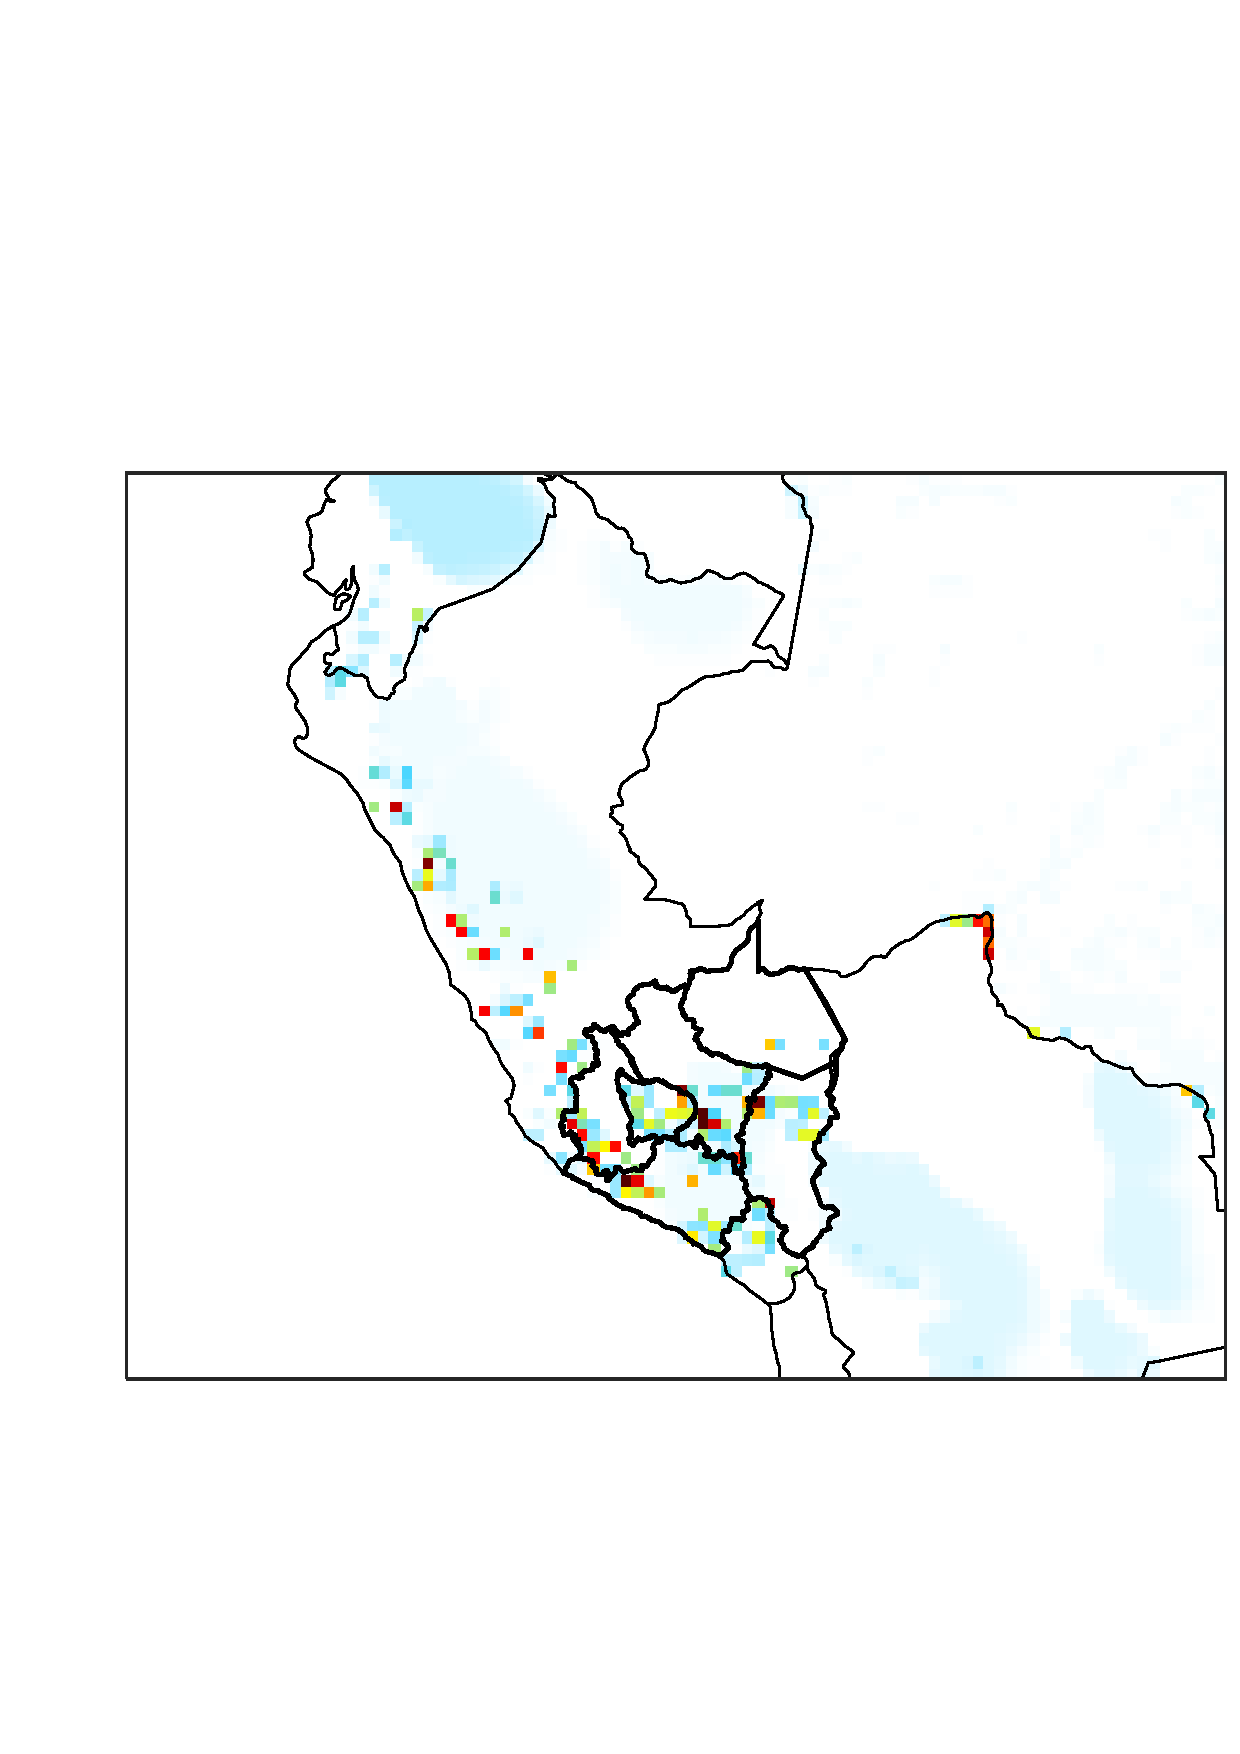
\includegraphics[width = 0.8\linewidth]{templates/figures/Peru_Maps/GMA2018inventory025x025.pdf}}\\
\subfloat[GEOS Chem Grid]{\includegraphics[width = 0.8\linewidth]{templates/figures/Peru_Maps/GMA2018inventory2x25.pdf}}

\end{tabular}
  

\captionof{figure}[Maps showing how the GMA2018 emission estimates for the year 2015 were distributed for Peru before re-griding (a) and after re-gridding to the \gc grid (b)]{Maps showing how the GMA2018 emission estimates for the year 2015 were distributed for Peru before re-griding (a)\cite{steenhuisen_development_2019} and after re-gridding to the \gc grid (b) }
\label{fig:GMA2018}
\end{figure}
\FloatBarrier
\end{flushleft}


\begin{table}[H]
\caption{Table showing the different GEOS-Chem simulations used in the analysis}
    \label{tab:all_geos_chem_simulations}
\begin{tabular}{lcp{0.5\linewidth}}

\textbf{Simulation Name}    &  Resolution       & \textbf{Description Estimate}                             \\
\hline
Base (ASGM=ON)              & 2.0$\times$2.5        & All Hg anthropogenic emission sources are turned on  \\
No ASGM (ASGM=OFF)          & 2.0$\times$2.5        & All ASGM emissions are turned off                     \\
Mdd                         & 2.0$\times$2.5        & Emissions from the \gc grid box located in  Madre de Dios  were scaled up by a factor of 2 \\

Apr                         & 2.0$\times$2.5        & Emissions from the \gc grid box located in Apurimac were scaled down by a factor of 0.5\\

Aqp                         & 2.0$\times$2.5        & Emissions from the \gc grid box located in Arequipa department were scaled up by a factor of 2\\

Npun                        & 2.0$\times$2.5        & Emissions from the \gc grid box located in the northern region of Puno were scaled up by a factor of 2 \\

Spun                        & 2.0$\times$2.5        & Emissions from the \gc grid box located in the southern region of the Puno were scaled up by a factor of 2 \\
\hline
\end{tabular}
\centering
\end{table}

\newpage
\subsection{Simulated Atmospheric Mercury Concentration Signals}\label{c3_simulated_atmospheric_hg}
\begin{flushleft}
The relationship between the \hg emissions from a specific grid box and the \gc simulated atmospheric \hg concentration at distant points from the emissions source is assumed to be defined by a linear function. This means that an increase in emissions is expected to increase the \hg concentration. Consequently, the relationship between emissions and concentrations can be represented by the following equation:


\begin{equation}
\label{doublingSig}
Hg^0_{sig(region)}=Hg_{m_0}+\small\frac{(Hg_{m_1} -Hg_{m_0})}{(m_1 -m_0)}(m_{(region)} -m_0)
\end{equation}
where:
\end{flushleft}

\begin{description}[leftmargin=!,labelwidth={5 em}]
    \item [$region$] is the location of the emission source within the case study region.
    \item [$Hg^0_{sig(region)}$] is the simulated \hg concentration at the observation site due to $m_{(region)}$ at the grid box in the specific $region $ of interest.
    \item [$Hg_{m_0}$] is the Hg concentration  at the observation site generated by the Base (ASGM =ON) simulation. 
    \item [$Hg_{m_1}$] is the Hg concentration  at the observation site generated by the $i^{th}$ region simulation $i$=Mdd,Apr, Aqp,Npun,Spun. 
    \item [$m_1$] is the amount of emissions in tons after scaling the emissions from a specific grid box.
    \item [$m_0$] is the amount of emissions in tons before scaling the emissions from a specific grid box.
\end{description}


% \begin{flushleft}
% $Hg_{sig(region)}$ gives the Hg concentration signal in the atmosphere that results from a unit change in the tonnes of emissions from a specific grid box. Therefore, $Hg_{sig(region)}$ was used to investigate the sensitivity of the observations to the different amounts of additional ASGM Hg emissions and the regional grid boxes. The Hg concentration in the atmosphere that results from a specific change in emissions from a particular grid box was calculated using Equation \ref{ysignal} below.
% \begin{equation}
% \label{ysignal}
% \small{Hg_{m(region)}} =Hg_{sig(region)}(m-m_o), 
% \end{equation}
% where:
% \end{flushleft}


% \begin{description}[leftmargin=!,labelwidth={1.5 em}]
    
%     \item [$m_0$] is the GMA 2018 ASGM emissions estimate in metric tonnes for the particular grid box corresponding to a place in the case study region
    
%     \item [$m$] is the amount of emissions, in metric tonnes, from a grid box required to produce $Hg_{m}$ concentration in the atmosphere
% \end{description}




% \begin{flushleft}
% For each grid box in the case study region, the emissions were modified from their original GMA 2018 estimates to new values based on Hg emission estimates produced by the Artisanal Gold Council(AGC)
% \end{flushleft}

\subsection{Observation Site Selection}\label{c3_site_selection}

\begin{flushleft}
TGM and GEM observation data from different locations in Latin America were analyzed and compared to the \gc simulated \hg concentrations for those sites in Chapter 2. The \gc predictions for ASGM contributions to atmospheric Hg concentration were higher at the CHC, making it an excellent candidate to use as a reference for comparison with the modified \gc Hg concentration predictions. Moreover, this site is the closest monitoring site to Peru hence it is expected that it would be more likely to detect atmospheric \hg changes that result from the changes in Hg emissions from the case study region. The time series of the observed concentration at the CHC station between July 2014 and January 2016 is shown in Figure \ref{fig:chc_time_series}.
\end{flushleft}

\begin{figure}[H]
  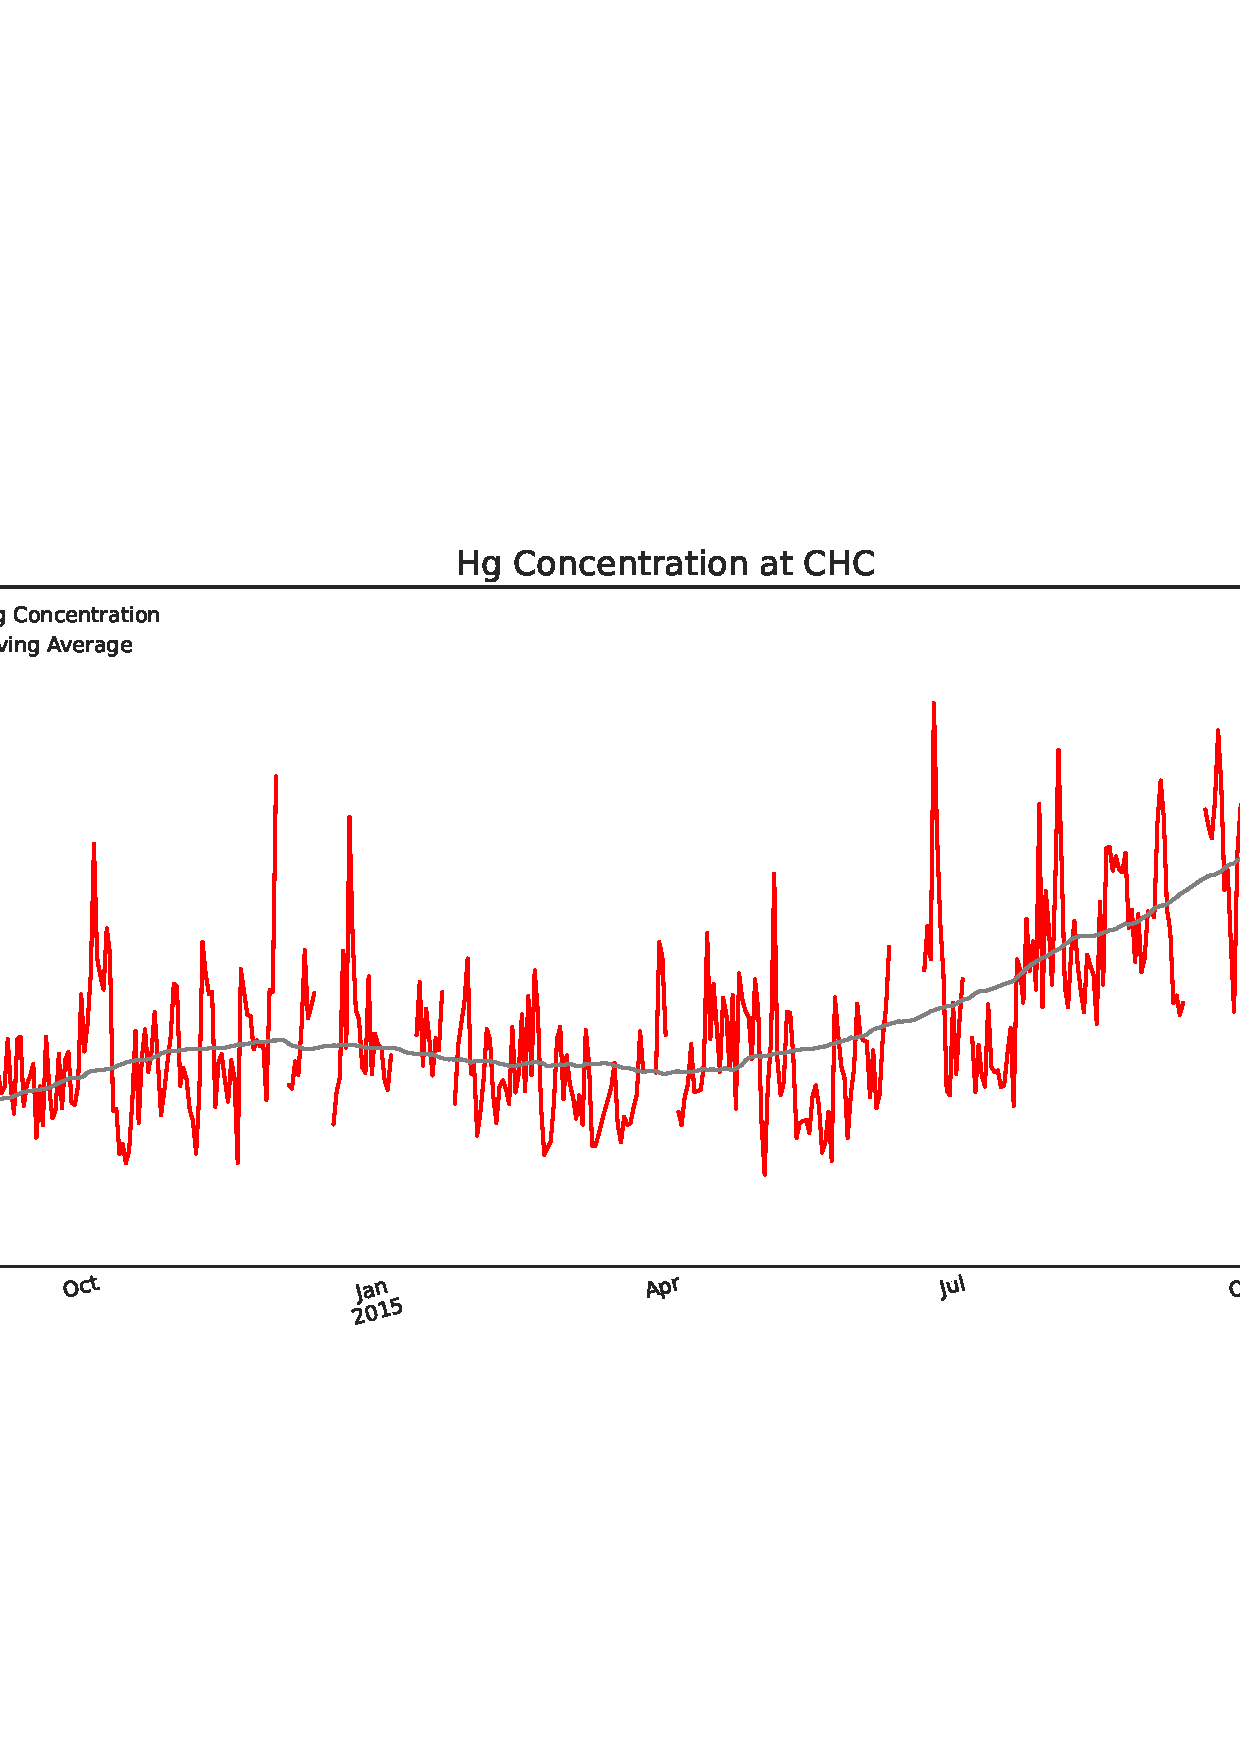
\includegraphics[width=\textwidth]{templates/figures/GMOS_Sites/ObsTimeSeries.pdf}
 
  \caption[The average daily TGM concentration at CHC in ng m\textsuperscript{-3} as a function of time over the measurement period from July 2014 to January 2016.]{The average daily TGM concentration at CHC in ng m\textsuperscript{-3} as a function of time over the measurement period from July 2014 to January 2016\cite{koenig_seasonal_2021}. The daily average concentration is indicated by the red line, while the grey line shows the 120-day moving average, which highlights the upward trend in the daily averages}
  \label{fig:chc_time_series}
  \centering
\end{figure}
\FloatBarrier
\begin{flushleft}

The detailed characteristics of the observations over this measurement period were described in Koenig et al.\cite{koenig_seasonal_2021}; hence my analysis focused on using the observation TGM data to evaluate the performance of the GEOS-Chem model in predicting the \hg based on the input \hg emission inventories. As shown in Figure \ref{fig:chc_time_series}, the TGM concentration at CHC showed an upward trend, which Koenig et al. (2021) attribute to El Ni\~no-Southern Oscillation (ENSO)\cite{koenig_seasonal_2021}. As a result, they categorized the measured TGM concentrations in the atmosphere at the CHC site as normal conditions (NC), 2014-07 to 2015-05, and ENSO conditions from 2015-06 to 2016-01. To reduce the number of records associated with ENSO, I limited my analysis to one year's worth of data from 2014-07 to 2015-07.
\end{flushleft}

\subsection{ Inverse Modelling with Markov Chain Monte Carlo}\label{c3_mcmc}
\begin{flushleft}
    Inverse modeling is described by Brasseur, and Jacob \cite{brasseur_modeling_2017} as a method for quantifying variables that drive a physical system using observations. Accordingly, the variables are statistically optimized based on the observational and other information available. Variables we wish to optimize are called state variables and assembled into a state vector $x$. In the same way, the observations are assembled into an observation vector $y$. The forward model $F$ of the physical system describes the relationship between $x$ and $y$:

    \begin{equation}
\label{inverse_model}
y=F(x,p) + \epsilon_0
\end{equation}
where:\\
\begin{description}[leftmargin=!,labelwidth={3 em}]
    \item [$p$] contains all variables in the model that we will not optimize as part of the inversion
    \item [$\epsilon_0$] a vector of observations errors, which includes errors from measurements, the forward model, and model parameters 
\end{description}
 Forward models describe the effects of the system as functions of the cause $x$, usually by using equations that describe the system's physics. The cause ($x$) can be quantified via inversion of the model based on the effect ($y$). Moreover, $x$ is estimated with some statistical error when $\epsilon_0 \neq 0$ is present. The solution for $x$ is called the optimal estimate, posterior estimate, or retrieval \cite{brasseur_modeling_2017}. 
 \end{flushleft}

\begin{flushleft}
    The uncertainty in obtaining $x$ from $y$ requires us to consider constraints on the value of $x$ called priors that could reduce the error on the optimal estimate.  We generally use the prior estimate $x_A$ as a constraint, representing our best estimate of $x$ before the observations. It has some error $\epsilon_A$. As a result, the ideal estimate must consider the relative information given by the observations $y$ and the prior estimate $x_A$. The error statistics of the estimates $\epsilon_O$ and $\epsilon_A$. In inverse modeling, we can analyze the relative importance of observations and prior knowledge. In this way, it provides insight into the effectiveness of an observing system in constraining $x$\cite{brasseur_modeling_2017}.

    \end{flushleft}

\begin{flushleft}
For this analysis, we use the measured Hg concentration (observation vector $y$) to constrain the  emissions from grid boxes in the case study region (state vector $x$). The forward model is given by the linear combination of the signals generated by the GEOS-Chem model as shown in Equation \ref{Hg_conc} below:

\begin{align}
\begin{split}\label{Hg_conc}
Hg_{conc}= {}&Hg_{m(MdD)}+ Hg_{m(S-Puno)} + Hg_{m(N-Puno)} + Hg_{m(Apr)}+ Hg_{m(Aqp)}\\
            & +Hg_{m_0} + \epsilon
\end{split}
\end{align}

where:
\end{flushleft}

\begin{description}[leftmargin=!,labelwidth={5 em}]
    \item [$Hg_{m(MdD)}$] is the Hg concentration signal resulting from emissions from the Madre de Dios (MdD) grid box
    \item [$Hg_{m(S-Puno)}$] is the Hg concentration signal resulting from emissions from the South Puno (S-Puno) grid box
    \item [$Hg_{m(N-Puno)}$] is the Hg concentration signal resulting from emissions from the North Puno (N-Puno) grid box
    \item [$Hg_{m(Apr)}$] is the Hg concentration signal resulting from emissions from the Apurimac (Apr) grid box
    \item [$Hg_{m(Aqp)}$] is the Hg concentration signal resulting from emissions from the Arequipa (Aqp) grid box
    \item [$Hg_{m_0}$] is the baseline Hg concentration signal.
    \item [$\epsilon$] is the error
\end{description}

\begin{flushleft}
Each of the $Hg_{m(region)}$ terms of Equation \ref{Hg_conc} represent signals from the different departments are calculated using Equation~\ref{doublingSig} an the form the parameter vector $p$. The $m_{(region)}$ terms are the only unknowns and the equation can be expanded to isolate the terms with $m_{(region)}$, which is the parameter we are optimizing for in the inverse modeling method. The expanded form of Equation \ref{Hg_conc} is shown below:

\begin{align}
\begin{split}\label{Hg_cons_expanded_form}
Hg_{conc}={}& (m_{(MdD)}Hg_{sig_{(MdD)}} -m_oHg_{sig_{(MdD)}})+ (m_{(S-Puno)}Hg_{sig_{(S-Puno)}} -m_oHg_{sig_{(S-Puno)}}) \\
            &+ (m_{(N-Puno)}Hg_{sig_{(N-Puno)}} -m_0Hg_{sig_{(N-Puno)}}) + (m_{(Apr)}Hg_{sig_{(Apr)}} -m_oHg_{sig_{(Apr)}}) \\
            &+ (m_{(Aqp)}Hg_{sig_{(Aqp)}} -m_oHg_{sig_{(Aqp)}})+Hg_{m_0}
\end{split}
\end{align}

Since the values of $m_{(region)}$ are the state variable we want to estimate, they can be represented as $\theta_i=m_{(region)}, i=1$ and the other terms, including the background concentration, are combined into one constant, C:

\begin{equation}
\begin{aligned}
    Hg_{conc}  & = \theta_0C  + \theta_1Hg_{sig_{(MdD)}}+ \theta_2Hg_{sig_{(S-Puno)}} +  \theta_3Hg_{sig_{(N-Puno)}} \\
                & \ \ \ \  +\theta_4Hg_{sig_{(Apr)}} +  \theta_5Hg_{sig_{(Aqp)}}
\end{aligned}
\end{equation}

\begin{align}
Hg_{conc} =\begin{bmatrix} C & Hg_{sig_{(MdD)}} & Hg_{sig_{(S-Puno)}} &Hg_{sig_{(N-Puno)}} &Hg_{sig_{(Apr)}} &Hg_{sig_{(Aqp)}}\end{bmatrix} \times 
            \begin{bmatrix} \theta_0 \\ \theta_1 \\ \theta_2\\ \theta_3\\ \theta_4\\ \theta_5  \end{bmatrix}
\end{align}
where $\theta_0=1$ and $Hg_{conc}$ is the modeled Hg concentration at the observation site of interest.
\end{flushleft}


\begin{flushleft}
The Markov-Chain Monte Carlo (MCMC) is a valuable sampling method for fitting models to data\cite{hogg_data_2018}. We apply the MCMC to constrain ASGM Hg emissions from the case study region in Peru.  The model is generated by a set of parameters and emissions, and we aim to sample from the parameters that best fit our data. The MCMC compares the modeled concentrations to the observed data using metrics such as the \nft confidence interval, mean, and the \iq. The MCMC models the given data by sampling around optimum values from the posterior distribution. The MCMC is a Bayesian approach; hence it requires the definition of priors on the parameters of interest. The priors encode information that we already know of the system. The probability of the model given the observed data is given by the posterior probability, $P(\theta|D)$, which is calculated using the Bayes theorem:

\begin{equation}
\label{bayes_eq}
P(\theta|D)=\frac{P(D|\theta)P(\theta)}{P(D)}
\end{equation}
where:
\end{flushleft}

\begin{description}[leftmargin=!,labelwidth={3 em}]
    \item [$P(D|\theta)$] is the likelihood which is the probability of the data given the model
    \item [$P(\theta)$] is the prior, which is the probability of the model and 
    \item [$P(D)$] is the evidence which is the probability of the data.
\end{description}

Bayes’ theorem relates posterior the probability distributions of parameters ($f_{post}(\theta, D)$) to the likelihood function ($f(D | \theta)$) and prior knowledge of the parameter distributions ($f_{prior}(\theta)$)

\begin{flushleft}
The MCMC enables the estimation of the sampling of the posterior distribution, which is the left-hand side of Equation~\ref{bayes_eq} by directly computing $P(\theta)$ and $P(D|\theta)$, and their product, for a very large ensemble of values of $\theta$ sampling strategically the n-dimensional space defined by the dimension of $\theta$\cite{brasseur_modeling_2017}. At each stage of MCMC sampling, a new parameter set $(\theta^{k+1})$ is drawn in the vicinity of the previous parameter set $(\theta^{k})$, that is from a normal distribution with $(\theta^{k})$, as the mean. The posterior probability of the new parameter set is calculated and compared to the previous set $(r = \frac{f^{k+1}}{f^k})$. If $r$ is greater than 1, the sample set is accepted, and if r is less than 1, the sample set is accepted with probability $r$ (and rejected with probability $1-r$). If the new parameter set is rejected, we retain the previous parameter set $(\theta^{k+1}= \theta^k)$. This procedure is repeated for 1000 samples. We use these samples to compute summary statistics on the posterior distributions of the parameters. 
\end{flushleft}

% \begin{align}
% \begin{split}\label{model_definition}
% \hat{y}= {}&Hg_{m(MdD)}+ 
% \end{split}
% \end{align}



\section{Results and Discussion}\label{c3_results}
\subsection{National vs. Global Mercury Inventory}
Figure \ref{fig:agc_vs_gma18} compares ASGM Hg emissions estimates from two different bottom-up inventories regrided to the GEOS-Chem 2$\times$2.5 grid used in the simulations in this study. The GMA 2018  estimates of Hg emissions from ASGM activities in Peru for 2015 as distributed by Steenhuisen and Wilson\cite{steenhuisen_development_2019} are shown in Figure \ref{fig:agc_vs_gma18},(a). Furthermore, Figure \ref{fig:agc_vs_gma18},(b) represents my interpretation of how the Peru ASGM Hg emissions estimates from the AGC's inventory\cite{agc_reporte_2017} would be mapped on to the GEOS Chem Grid. The estimates for the total ASGM emissions from Peru are almost similar in both inventories, 110.4 t/y in the GMA 2018 and 108.74 t/y in the AGC national inventory.

% \begin{figure}[H]
% \centering

% \begin{tabular}[H]{cc}

% \subfloat[]{\includegraphics[width = 0.5\linewidth]{templates/figures/Peru_Maps/GMA2018inventory2x25Peru.pdf}}
% \subfloat[]{\includegraphics[width = 0.5\linewidth]{templates/figures/Peru_Maps/AGCinventory2x25Peru.pdf}}\\


% \end{tabular}
\begin{figure}[H]
\centering
  \includegraphics[width=\textwidth]{templates/figures/Peru_Maps/comparison_AGC_GMA18.pdf}  

\captionof{figure}[The AGC Peru National ASGM Hg emissions inventory vs. the GMA2018 ASGM Hg emissions inventory for 2015 ]{The AGC Peru National ASGM Hg emissions inventory as published in \cite{agc_reporte_2017} and regridded to the GEOS-Chem 2$\times$2.5 grid resolution is shown in (a).How the ASGM Hg emissions in Peru were distributed in two bottom-up inventories. The GMA2018 ASGM Hg emissions inventory for 2015 as distributed in Steenhuisen and Wilson \cite{steenhuisen_development_2019} and regridded  to the GEOS-Chem 2$\times$2.5 grid resolution is shown in (b).}
\label{fig:agc_vs_gma18}
\end{figure}
\FloatBarrier
\begin{flushleft}
The AGC's Peru national inventory attributed most of the ASGM Hg emissions to the South Eastern departments in the country\cite{agc_reporte_2017}. As seen in Table \ref{tab:agc_vs_gma18}, the Madre de Dios department is the largest source of Hg emissions, followed by Arequipa, Puno, Ayacucho, Cusco, respectively. The rest of Peru together contributes about 0.98 tonnes of Hg emissions annually. In contrast with the AGC's method, Steenhuisen, and Wilson\cite{steenhuisen_development_2019} based the Hg emissions spatial distribution on a proxy based on the likelihood of gold occurrence in soils, sediments, and bedrock and knowledge of actual ASGM activity. For Peru, they used the global alluvial gold map and a (gold) mining concessions dataset for Peru.
\end{flushleft}


\setlength{\tabcolsep}{5pt}
\begin{table}[H]
  \begin{center}
    \caption[Comparison of Peruvian ASGM Hg emissions estimates from the GMA2018 inventory for 2015 and estimates from the AGC national inventory of ASGM Hg emissions]{Comparison of Peruvian ASGM Hg emissions estimates from the GMA2018 inventory for 2015 and estimates from the AGC national inventory of ASGM Hg emissions from the case study region. The emissions units are tons/year, and the right-most column shows the percentage difference between the AGC and GMA 2018 Hg emissions estimates. }
    \label{tab:agc_vs_gma18}
    \begin{tabular}{lrrr}
       %<-- added & and content for each column
      
    \textbf{Region}     & \textbf{AGC}      & \textbf{GMA 2018}             & \textbf{Percentage Difference}       \\
                        & (t$\cdot y^{-1}$) & (t$\cdot y^{-1}$)                    &        (\%)\\
\hline    
    Madre de Dios       & 54.46             & 1.39                          &    -97.45       \\
    Puno                & 19.37             & 19.42                         &    +0.26     \\
    Arequipa            & 23.86             & 18.99                         &    -20.41       \\ % <--
    Apurimac            & 0.03              & 19.32                         &    +64300.00    \\
    Ayacucho            & 9.15              & 8.99                          &    -1.75           \\ % <--
    Cusco               & 0.89              & 0.04                          &    -95.50           \\
    Rest of Peru        &  0.98             & 42.25                         &    +4211.22        \\
   
    \hline
    \textbf{Total}           &108.74           & 110.40      &        \\
    \end{tabular}
  \end{center}
\end{table}
\begin{flushleft}
The Madre de Dios department is a well-known ASGM hotbed in Peru, and within the Amazon region hence the GMA 2018 estimate of Hg emissions of 1.39 t/y can be easily identified as inaccurate. Moreover, Diringer et al.\cite{ding_w_dynamic_2020} estimated that the amount of Hg used in ASGM in Madre de Dios was at least 30 tons per year, which also undermines the GMA 2018 estimate. 

% The AGC's inventory gives a baseline of the amount and distribution of ASGM Hg emissions at the national level but does not show the influence of the emissions at the regional and global levels. On the other hand, the global inventory is a source of information about local, regional and global emissions. 
\end{flushleft}

\begin{flushleft}
    As discussed in Chapter 2, the \on model did not reproduce atmospheric Hg concentrations, and the above comparison of global and national inventories was conducted to determine the role played by emission inputs in the poor model's replication of observed atmospheric concentrations. In light of the uncertainty in the inventories of Hg emission estimates and the above findings about the differences in the inventories, it was hypothesized that the poor predictions of \on may be the result of incorrect emission parameterization in \gc. Following are the results of scaling the emissions from the departments in the case study and comparing them with observations. A top-down estimate of Hg emissions for Peru is also provided.
\end{flushleft}

\subsection{GEOS-Chem Predictions vs. Observations at Chalcataya}\label{c3_geos_chem_vsobs}
\begin{flushleft}
The comparison of the \gc predicted \hgc to observed TGM at CHC for the one year from 2014/07/03 to 2015/07/03 is shown in Table \ref{tab:ModelvsObsStats}. The metrics being compared on the table are the mean ($\mu$), standard deviation ($\sigma$), interquartile range (\iq), Spearman correlation ($r_s$) and Pearson correlation ($r$).The mean \hg concentration produced by the \off  was within 1\% of the observed TGM concentration as seen in Table \ref{tab:ModelvsObsStats}. On the contrary, the average \hg produced by the \on overestimated the mean by 29\%.
\end{flushleft}
\setlength{\tabcolsep}{3.5pt}
\begin{table}[H]
  \begin{center}
    \caption[Characteristics of observed and modeled Hg concentration in CHC.]{Characteristics of observed and modeled Hg concentration in CHC where $\mu$ is the annual average Hg concentration, $\sigma$ is the standard deviation, \iq is the interquartile range, $r_s$ is the Spearman correlation, $r$ is the Pearson correlation }
    \label{tab:ModelvsObsStats}
    \begin{tabular}{lccccc}
       %<-- added & and content for each column
      
                            & $\mu$                 & $\sigma$              & \iq                & & \\
                            &  (ng m$^{-3}$)/year)  & (ng m$^{-3}$)/year)   & (ng m$^{-3}$)/year)   & & \\
     \cmidrule{2-4}
     Observations           & 0.90                  & 0.16                  & 0.18                  &  & \\
     \textbf{Simulations}   &                       &                       &                       &\textbf{$r_s$} &\textbf{$r$} \\ %
      \hline
      No ASGM (ASGM=OFF)    & 0.91                  & 0.060                  & 0.11                  & 0.17          & 0.14        \\ 
      Base (ASGM=ON)        & 1.2                 & 0.14                  & 0.20                  & 0.12         & 0.27        \\ % <--
    \end{tabular}
  \end{center}
\end{table}
\FloatBarrier
\begin{flushleft}
   Figure \ref{fig:ModelvsObsNstats} shows a detailed comparison of the simulated \hg concentration and the observed TGM concentration at CHC. The observations (in red) are plotted as a function of time in plots (a) and (c) with the \off (in green) in plot (a)  and the \on in (blue) in plot (c). 
   The low correlation between both modeled \hg concentrations and the observations is also evident in the scatter plots in (b) and (d).  However, the \on closely approximates the variability (defined by the standard deviation)  in the observed Hg concentration as its standard deviation is only 12.5\% less than the  observation standard deviation, yet the \off standard deviation is 62.5 \% less than the observation standard deviation. While here, the dataset has been truncated to one year from 2014/07/03 to 2015/07/03, this study follows Chapter 2, where the entire CHC dataset was compared with the modeled \hgc at CHC. 
\end{flushleft}
\begin{figure}[H]
  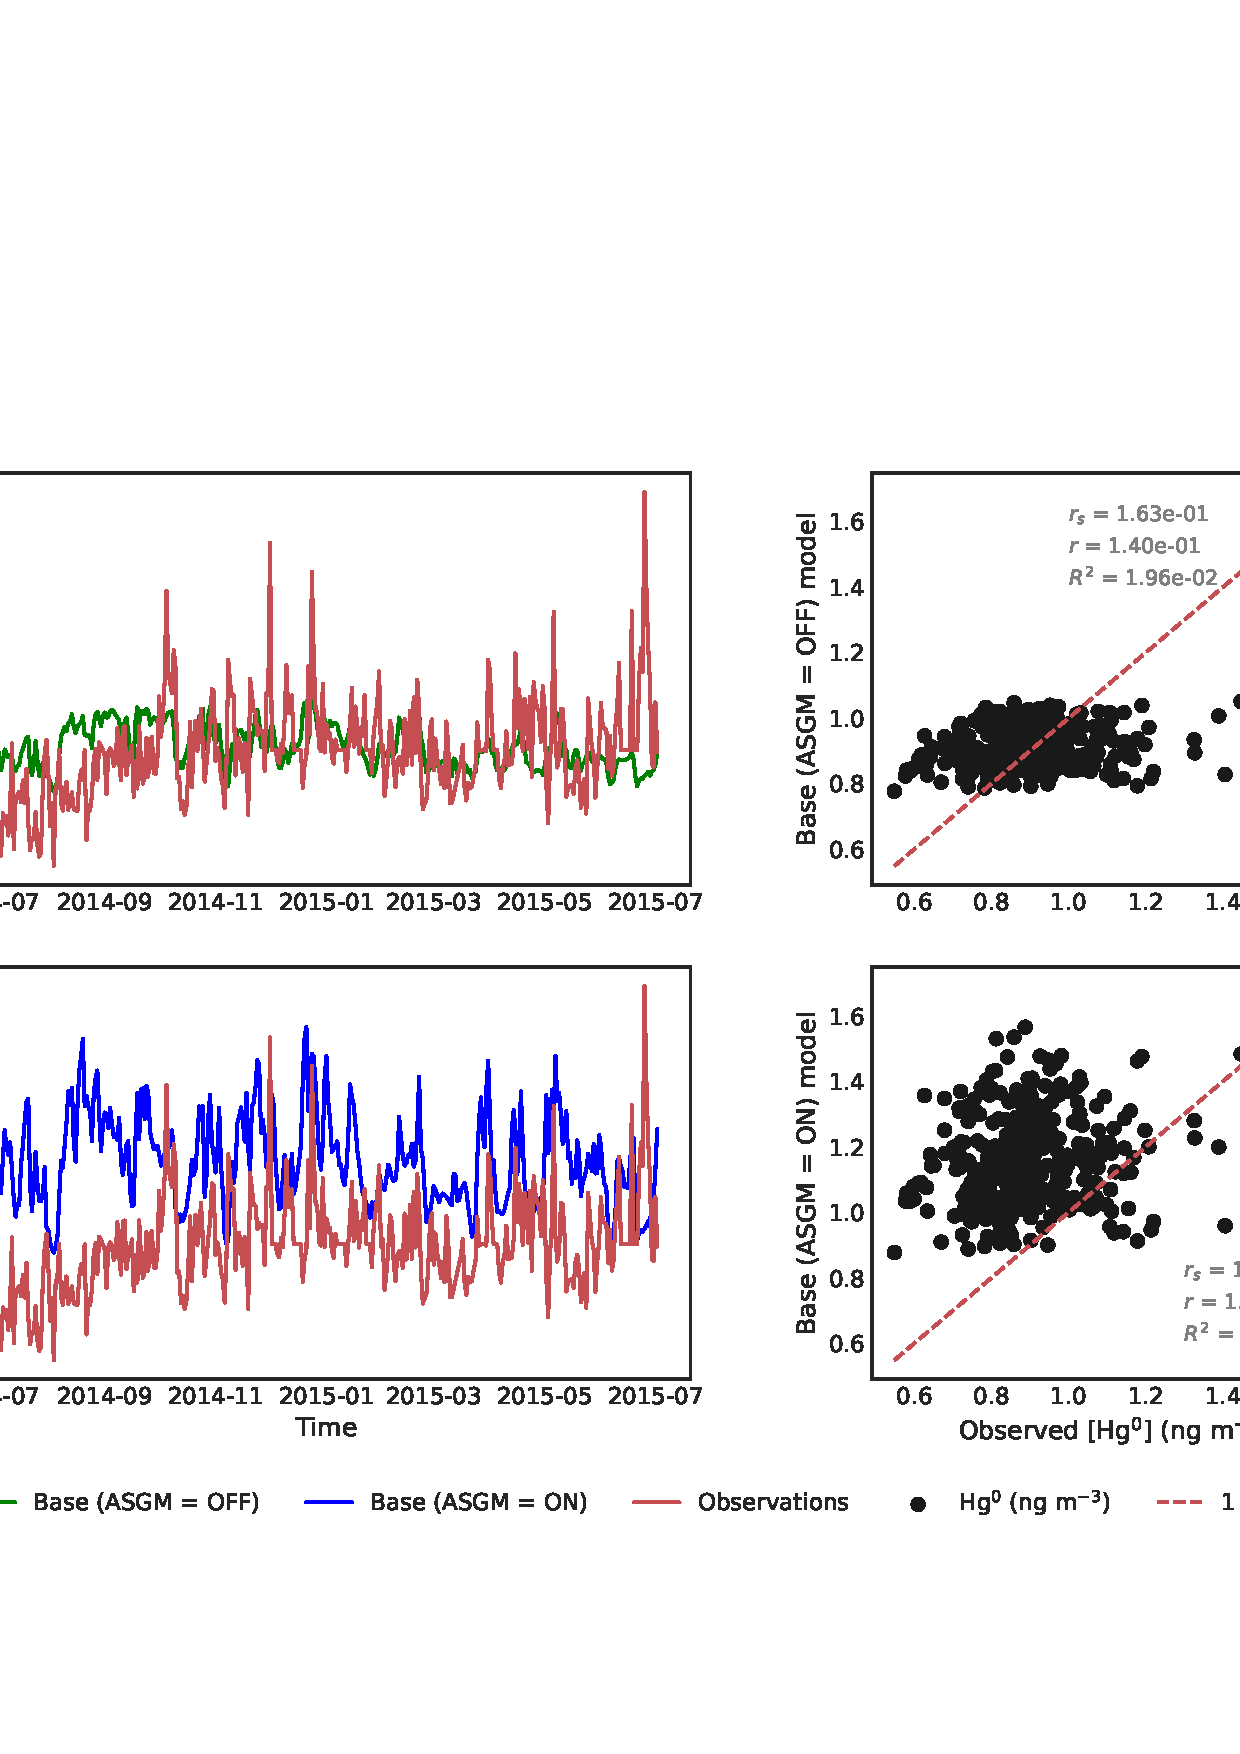
\includegraphics[width=0.85\textwidth]{templates/figures/ModelvsObs/TimeSeriesNsactter_obsVmodel_v1.pdf}
  \centering
  \caption[Hg concentration in the atmosphere as a function of time and scatter plots of modeled concentration as a function of the observations]{The observations (in red) are plotted as a function of time in plots (a) and (c) with the \off (in green) in the plot (a) and the \on in (blue) in the plot (c). Analysis of the observed Hg concentrations vs. the \off  shows how the modeled mean closely approximates the observed mean and poorly estimates the daily variability, as shown by the difference in the size of the daily spikes of the Hg concentrations. The scatter plots in (b) and (d) represent the modeled \hg  as a function of the measured TGM concentration.}
  \label{fig:ModelvsObsNstats}
\end{figure}
\FloatBarrier

\begin{flushleft}
    Even though GEOS-Chem closely approximated the mean Hg concentrations at CHC in the \off, the Spearman ($r_s$) and Pearson ($r$) correlations between the modeled and observed concentrations were very low at 0.17 and 0.144, respectively. Moreover, the coefficient of determination, $R^2$ between the observed and modeled concentrations in \off case was almost zero at 0.0207. This is in line with the general result in Chapter 2 that the model poorly estimates the observed Hg emission concentrations in the atmosphere. Brasseur and Jacob (p.471)\cite{brasseur_modeling_2017} argue that in cases where a model captures the observed means but not the observed variability, the mean may be wrongly interpreted \cite{brasseur_modeling_2017}. In line with Brasseur and Jacob's argument, the wrong interpretation of the \off mean is encapsulated in the direct comparison of the \off and \obsC.  This is because Hg concentrations in the atmosphere captured in \obsC are affected by ASGM emissions near CHC. Moreover, a poor definition of dry deposition or vegetation uptake in the model further leads to underestimating observed Hg concentrations.  
\end{flushleft}

\begin{flushleft}
The \on reproduces the \iq and 95th \% confidence interval better than it reproduces the mean, as seen in Figure \ref{fig:density_plots_noASGM_vs_ASGM_vsObs}. Density plots of the modeled and observed Hg concentration at Chalcataya are shown in Figure \ref{fig:density_plots_noASGM_vs_ASGM_vsObs}. In (a), the actual distributions for the two simulations and the observations are plotted where the observed TGM concentration distribution is shown in red, the distribution of the \hgc predicted by the \off is shown in green, and that produced by the \on is shown in blue. Figure \ref{fig:density_plots_noASGM_vs_ASGM_vsObs} (b) shows the identical distributions to (a) after standardization by subtracting the mean in each distribution to see how the shapes of the distributions compare with each other.  
\end{flushleft}



\begin{figure}[H]
\begin{tabular}[H]{cc}
\subfloat[]{\includegraphics[width = 0.45\linewidth]{templates/figures/ModelvsObs/06-12-22_models_vs_observations_density-plot.pdf}} &
\subfloat[]{\includegraphics[width = 0.45\linewidth]{templates/figures/ModelvsObs/06-12-22_models_vs_observations_density-plot_std.pdf}}
\end{tabular}
\centering
\captionof{figure}[Density plots of the modeled and observed Hg concentration at Chalcataya.]{Density plots of the modeled and observed Hg concentration at Chalcataya. In (a), the actual distributions for the two simulations and the observations are plotted where the observed TGM concentration distribution is shown in red, the distribution of the \hgc predicted by the \off is shown in green, and that produced by the \on is shown in blue. In (b), the same distributions are shown after standardization by subtracting the mean in each distribution for easy comparison of the shapes of the distributions}
\label{fig:density_plots_noASGM_vs_ASGM_vsObs}
\end{figure}
\FloatBarrier
\begin{flushleft}
    Figure \ref{fig:density_plots_noASGM_vs_ASGM_vsObs}, b) shows how the \hgc produced by the \on have a distribution that is similar to the distribution of the observations in terms of standard deviation, \iq and \nft. The \off produced \modelc shows no instance of high \hg concentrations at CHC, and the high concentrations are only produced by the \on. These density plots inform us that ASGM emissions primarily influence the range of observed Hg concentrations in the atmosphere at CHC. Consequently, metrics such as the standard deviation, \iq, and \nft may lead to more informative comparisons between \modelc and \obsC than the mean.
\end{flushleft}
\newpage

\subsection{Comparison of Observations with Emission Modification}\label{c3_obs_v_modifications}
\begin{flushleft}
The sensitivity of the modeled \hgc at CHC to the changes in Hg emissions from each grid box in the case study region was investigated by finding the mean, \iq, and correlation between \modelc and \obsC as functions of the emissions from each specific grid box. Each plot in Figure \ref{fig:mean_of_signals_vs_emissions_per_site} shows the relationship between the mean of \modelc as a function of Hg emissions from the grid box corresponding to the respective region in the case study. For each plot, the emissions from one grid box are varied between  0 to 100 tons in increments of 10 tons, while the emissions from the other grid boxes are kept at their \on level. 
\end{flushleft}

\begin{flushleft}
 The means of \modelc for a given amount of Hg emissions from each grid box are compared to the red horizontal line. This red horizontal line indicates the value of the mean of \obsC (0.90), as presented in Table \ref{tab:ModelvsObsStats}.  Moreover, the blue dashed line shows the linear regression line for the values of \modelc as a function of the Hg emissions. All the plots show that the mean of the Hg concentration changes linearly with an increase in emissions and have a $R^2$ value of 1, which validates the linear assumption between emissions and concentrations. Furthermore, none of the blue dashed lines intersect the red line within the given emissions range, which also undermines the mean as a metric for comparing \modelc to \obsC.
\end{flushleft}
%____________________________________________Figure Start _______________________________________________
\begin{figure}[H]
\begin{tabular}[H]{cc}
\centering
\subfloat[South Puno]{\includegraphics[width = 0.45\linewidth]{templates/figures/individual_site_modifications/mean_Spun_sigs.pdf}} &
\subfloat[North Puno]{\includegraphics[width = 0.45\linewidth]{templates/figures/individual_site_modifications/mean_Npun_sigs.pdf}}\\
\subfloat[Arequipa]{\includegraphics[width = 0.45\linewidth]{templates/figures/individual_site_modifications/mean_Aqp_sigs.pdf}} &
\subfloat[Apurimac]{\includegraphics[width = 0.45\linewidth]{templates/figures/individual_site_modifications/mean_Apr_sigs.pdf}}\\
\subfloat[Madre de Dios]{\includegraphics[width = 0.45\linewidth]{templates/figures/individual_site_modifications/mean_Mdd_sigs.pdf}} & \subfloat{\includegraphics[width = 0.45\linewidth]{templates/figures/individual_site_modifications/mean_caption.pdf}}
\end{tabular}
\caption[Plots of regression of mean of \modelc as a function of Hg emissions amount]{ }
\label{fig:mean_of_signals_vs_emissions_per_site}
\end{figure}
\FloatBarrier
%____________________________________________Figure End _______________________________________________

\newpage
\begin{flushleft}
    Contrary to Figure \ref{fig:mean_of_signals_vs_emissions_per_site} where the relationships between the Hg emissions and the mean of \modelc have similar \rsq values (\rsq=1), the relationship between the \iq of \modelc  and the emissions from each grid box in Figure \ref{fig:iqr_vs_emissions_per_site} have different \rsq values. For each plot in Figure \ref{fig:iqr_vs_emissions_per_site}, the emissions from one grid box are varied between  0 to 100 tons in increments of 10 tons while the emissions from the other grid boxes are kept at their \on level. Even though the \rsq values are different, they are all above 0.85, which validates the linear assumption between the emissions and the \rsq values of the Hg concentration. The values of the \iq for a given amount of Hg emissions from each grid box are compared to the red horizontal line, which indicates the \iq of \obsC, (0.16) . 
    
\end{flushleft}
\begin{flushleft}
     All the lines showing the relationship between the \iq of \modelc and the emissions intersect the red line representing the \iq of \obsC. The Hg emissions value of the point of intersection between the regression line and the red line can be interpreted as what the emissions from the given grid box should be for the \modelc to match the \obsC. The actual values of the emissions can also be calculated using the regression equation given on each plot. 

\end{flushleft}

%___________________________________________Figure Start____________________________________________
\begin{figure}[H]
\begin{tabular}[H]{cc}
\centering
\subfloat[South Puno]{\includegraphics[width = 0.45\linewidth]{templates/figures/individual_site_modifications/iqrSpun_sigs.pdf}} &
\subfloat[North Puno]{\includegraphics[width = 0.45\linewidth]{templates/figures/individual_site_modifications/iqrNpun_sigs.pdf}}\\
\subfloat[Arequipa]{\includegraphics[width = 0.45\linewidth]{templates/figures/individual_site_modifications/iqrAqp_sigs.pdf}} &
\subfloat[Apurimac]{\includegraphics[width = 0.45\linewidth]{templates/figures/individual_site_modifications/iqrApr_sigs.pdf}}\\
\subfloat[Madre de Dios]{\includegraphics[width = 0.45\linewidth]{templates/figures/individual_site_modifications/iqrMdd_sigs.pdf}} & \subfloat{\includegraphics[width = 0.45\linewidth]{templates/figures/individual_site_modifications/iqrcaption.pdf}}
\end{tabular}
\caption[Plots of regression of \iq of \modelc as a function of Hg emissions amount]{}
\label{fig:iqr_vs_emissions_per_site}
\end{figure}
\FloatBarrier
%___________________________________________ Figure End ____________________________________________
\newpage
\begin{flushleft}
     
     Unlike in Figures \ref{fig:mean_of_signals_vs_emissions_per_site} and \ref{fig:iqr_vs_emissions_per_site}, the Pearson correlation coefficient ($r$) between the TGM concentration and \modelc has a negative trend in all the emissions scenarios. Int he concentxt of model obsevation comparison, the Pearson correlation coefficient characterizes how patterns in the observations are matched by patterns in the model\cite{brasseur_modeling_2017}. According to Brasseur and Jacob, values of $r$ near zero imply that the variability in the observations is controlled by processes that the model does not capture. Table \ref{tab:ModelvsObsStats} shows that $r$ of the \on is very low at 0.27. As in Figures  \ref{fig:mean_of_signals_vs_emissions_per_site} and \ref{fig:iqr_vs_emissions_per_site}, the emissions from the corresponding region are varied from 0 to 100 tons in increments of 10 tons for each plot in Figure \ref{fig:corr_vs_emissions}. 
     
      
\end{flushleft}

\begin{flushleft}
     For each emissions scenario, the correlation between the TGM concentration and \modelc is indicated by the black dot. The red horizontal line indicates the Pearson correlation between \obsC and the \on (0.27). The dashed blue line shows the regression line of the correlation between \modelc and \obsC as emissions from each grid box increase. It is evident that increasing the emissions from one region while keeping the emissions from other regions at the \on level did not lead to improvements to the extent to which the patterns in the observations are matched by the pattern in \modelc. However, the rate at which the correlation decreases may reveal information about the sensitivity of \modelc to the emissions from a specific region. For instance the shallow slope in the regression line for  the Madre de Dios scenarios may be an indicator that the emissions from Madre de Dios are underestimated.
     
\end{flushleft}


%___________________________________________Figure Start____________________________________________
\begin{figure}[H]
\begin{tabular}[H]{cc}
\centering
\subfloat[South Puno]{\includegraphics[width = 0.45\linewidth]{templates/figures/individual_site_modifications/corr_Spun_sigs.pdf}} &
\subfloat[North Puno]{\includegraphics[width = 0.45\linewidth]{templates/figures/individual_site_modifications/corr_Npun_sigs.pdf}}\\
\subfloat[Arequipa]{\includegraphics[width = 0.45\linewidth]{templates/figures/individual_site_modifications/corr_Aqp_sigs.pdf}} &
\subfloat[Apurimac]{\includegraphics[width = 0.45\linewidth]{templates/figures/individual_site_modifications/corr_Apr_sigs.pdf}}\\
\subfloat[Madre de Dios]{\includegraphics[width = 0.45\linewidth]{templates/figures/individual_site_modifications/corr_Mdd_sigs.pdf}} & \subfloat{\includegraphics[width = 0.45\linewidth]{templates/figures/individual_site_modifications/corr_caption.pdf}}
\end{tabular}
\caption[Plots of regression of correlation of \modelc as a function of Hg emissions amount]{ }
\label{fig:corr_vs_emissions}
\end{figure}
\FloatBarrier
%___________________________________________ Figure End ____________________________________________
\newpage

\begin{flushleft}
     This section has shown the effect of changing Hg emissions from individual grid boxes in the modeled \hgc at a distant active monitoring site like CHC. ASGM Hg emissions estimates of the from the different regions would be obtained graphically from each of the plots by identifying the point of intersection between the red horizontal line and the regressions line or solving the regression line equation. However, the range of these estimates would not be robust; hence following section presents the emission estimates generated using the MCMC, which accounts for emission changes from multiple regions. 

\end{flushleft}

\subsection{Estimating Emissions with Markov Chain Monte Carlo}\label{c3_mcmc_estimates}
Based on the \nft, the MCMC approach produced \hg emissions estimates within the range of bottom-up inventory estimates. The distributions of the estimates produced by the MCMC approach are shown in Figure \ref{fig:MCMC_estimates95th}. The box and whisker plots illustrate Hg0 emissions when the 95th percentile range is used to compare the modeled Hg0 concentration and the TGM concentration. In the box plots, the horizontal lines represent the emission estimates based on bottom-up inventories. Solid horizontal lines represent emission estimates from the GMA 2018 inventory \cite{united_nations_environment_programme_technical_2019,steenhuisen_development_2019}; dashed lines represent emission estimates from Peru's bottom-up inventory. In Table \ref{tab:MCMC_estimates}, we describe the mean estimates of emissions from these regions and their ranges \cite{agc_reporte_2017}.  

\begin{figure}[H]
  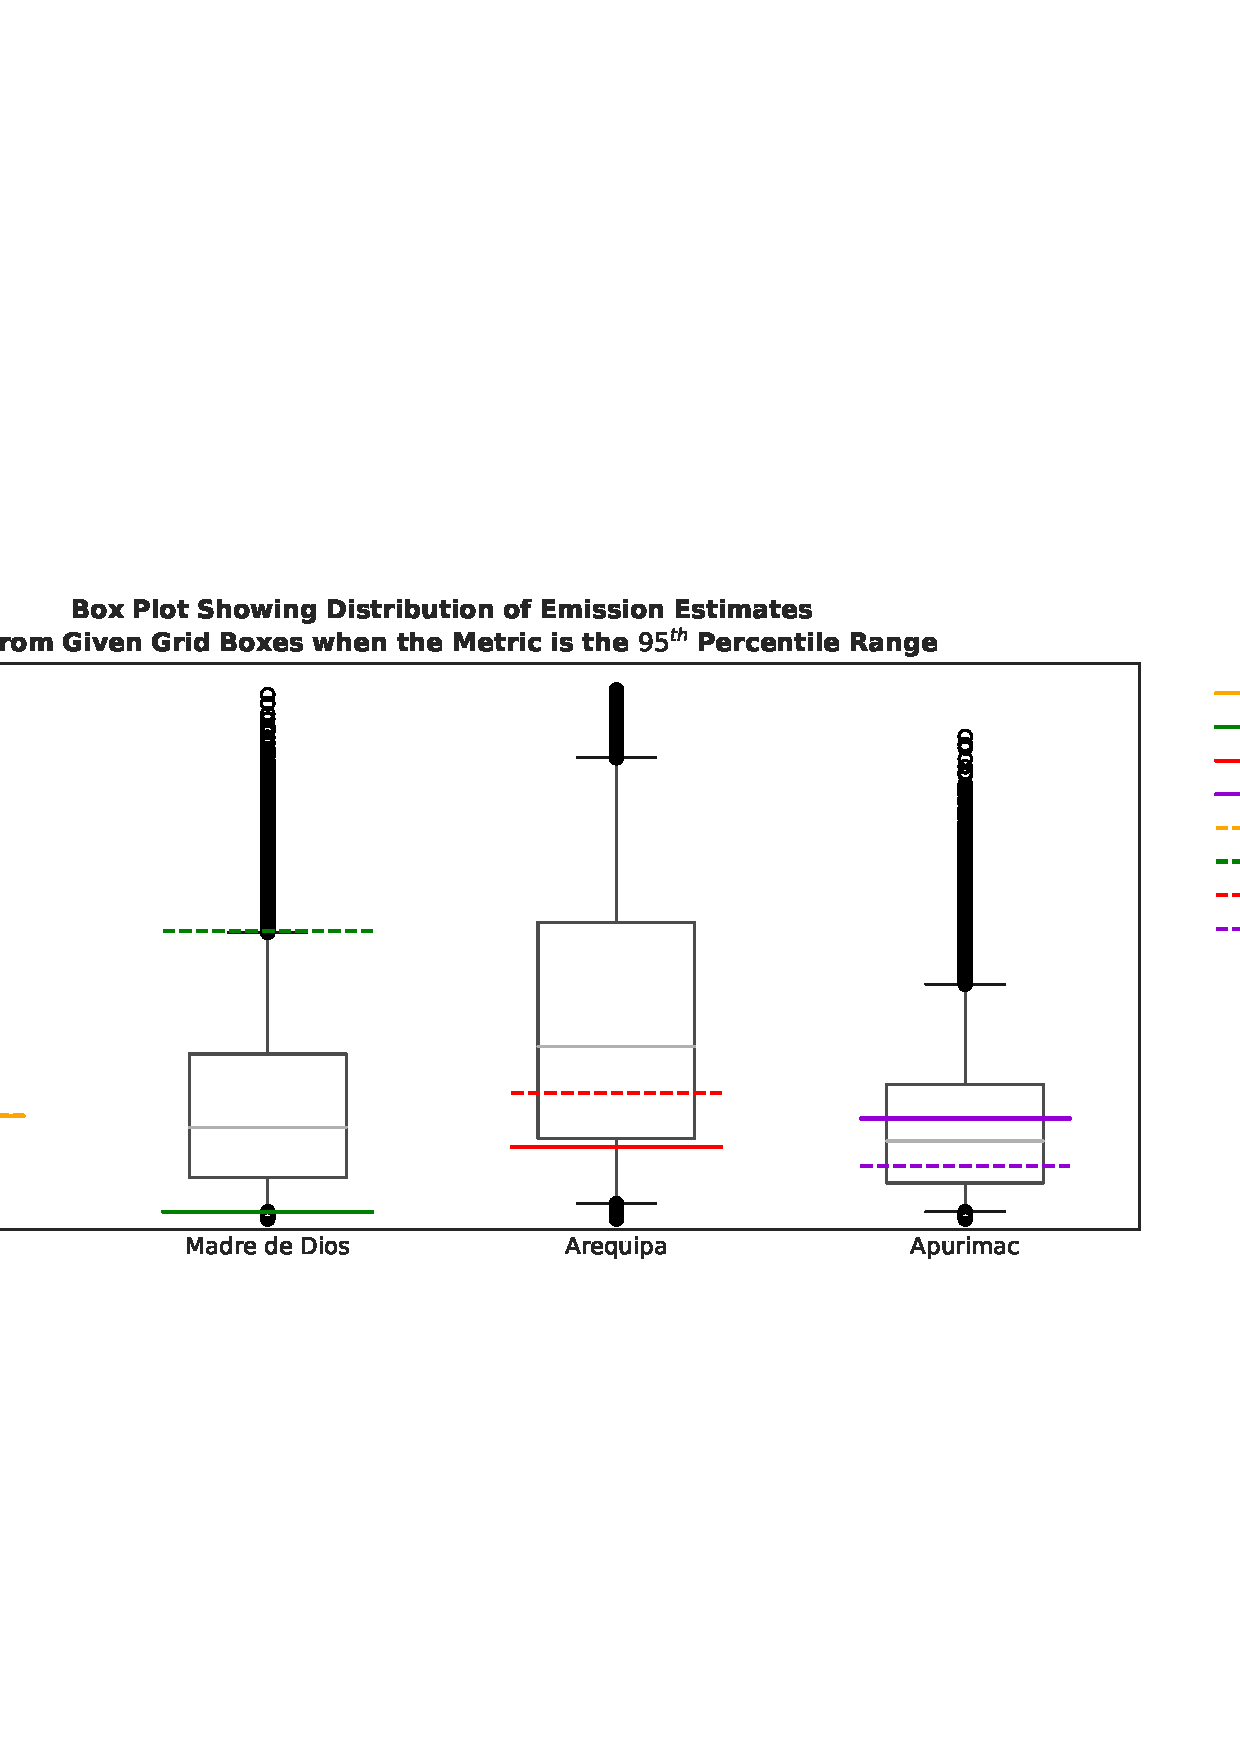
\includegraphics[width=\textwidth]{templates/figures/MCMC/MCMCMCMC_Estimates95th.pdf}
  \centering
  \caption[Emission Estimates when the $95^{th}$ percentile range is used as the metric to compare the model outputs to observations.]{Emission Estimates when the $95^{th}$ percentile range is used as the metric to compare the model outputs to observations. The horizontal lines representing the emission estimates from the bottom-up inventories are traced over the box plots. The solid horizontal lines represent the emission estimates from the GMA 2018 inventory \cite{united_nations_environment_programme_technical_2019,steenhuisen_development_2019} and the dashed lines represent the emission estimates from the bottom-up inventory published by the Artisanal Gold Council\cite{agc_reporte_2017}.}
  \label{fig:MCMC_estimates95th}
\end{figure}
\FloatBarrier

\begin{flushleft}
    These are the first ever top-down estimates of Hg emissions from ASGM activities.  Even though the ranges of the estimates are wide, they result from the uncertainty in the models and data we could access. Therefore, these results may be improved if more data from monitoring sites were available to constrain the emissions. Nevertheless, the top-down estimate of the total amount of ASGM Hg emissions under-predicts the GMA 2018 total estimate for Peru by a factor of 1.09 and the AGC estimate by a factor of 1.08. The comparison of the top-down ASGM Hg estimates with the bottom-up estimates is visualized in Figure \ref{fig:all_asgm_hgEstimates}. It is essential to highlight the Madre de Dios region's estimate of 21 tons/year of ASGM Hg emissions. This estimate is an improvement aligned with the literature about the high ASGM Hg emissions in the region. However, it is still a drastic underestimate compared to the AGC baseline ASGM Hg estimate for Madre de Dios.
\end{flushleft}    
\begin{table}[H]
\caption{Table showing the emission estimates for each of the grid boxes in the case study region when the $95^{th}$ percentile range is used as the metric to compare the model outputs to observations}
    \label{tab:MCMC_estimates}
\begin{tabular}{lcc}

\textbf{Region}        & \textbf{Emission Estimate (Mg)}  &     \textbf{Range of Estimate (Mg)}                      \\
\hline
Madre de Dios          & $21$                               & $1.36 - 54.12$\\

Apurimac               & $17$                               & $1.36 - 44.37$\\

Arequipa               & $37$                               & $2.88 - 87.14$\\

Puno                    & $25$                              & $5.85 - 51.05$\\
\hline
Total                  & $101$                            &  $11.45 - 236.69$ \\
\hline
\end{tabular}
\centering
\end{table}

\begin{figure}[H]
  \includegraphics[width=\textwidth]{templates/figures/all_asgm_hgEstimates.pdf}
  \centering
  \caption[Comparison of estimates of total ASGM Hg emissions from Peru ]{Bar chart shows the different estimates  of the total ASGM Hg emissions from Peru. The height of the bars indicates the estimated Total emissions, and the error in each estimate is shown by the error bars.}
  \label{fig:all_asgm_hgEstimates}
\end{figure}
\FloatBarrier

\begin{flushleft}

 Our study produced top-down estimates of ASGM Hg emissions for four Peruvian departments and thus the country's total ASGM Hg emissions estimates. Table \ref{tab:MCMC_estimates} shows Peru emits 101.23 tons of Hg annually, ranging from 11.45 tons to 236.69 tons. There is a wide range here, but it is a confidence interval based on the data and the uncertainty of the model discussed so far. The estimates would be improved if more relevant measurements of atmospheric Hg were used instead of just one-site data. Another potential source of refinement in the estimates may result from the model's improved parameterization of vegetation uptake discussed in Feinberg et al.(2022) \cite{feinberg_evaluating_202}.
  \end{flushleft}
  
  \begin{flushleft}
  Model improvements and more time series atmospheric Hg concentration data may enable us to use the mean as another constraint for producing \hg emission estimates.  Also, these results demonstrate that extreme values are vital for quantifying non-point sources like ASGM, where variability over time is somewhat unpredictable. The analysis in this chapter focused on a region in Peru where ASGM dominates. These top-down will be challenging to implement in areas where ASGM co-occurs with many point sources, such as Southeast Asia, where biomass and coal are burned simultaneously. Furthermore, the global resolution of GEOS-Chem is not particularly suitable for monitoring Hg in mountainous regions such as CHC. Future work may extend this method and this proof of concept using more satisfactory results focusing on the region. 
   \end{flushleft}
  
  \begin{flushleft}
  In addition to helping resolve the differences in global and national ASGM Hg emission estimates, the above analysis also provides a stronger foundation for answering the second question about how regional monitoring networks can improve the utility of models for MC effectiveness evaluations. Creating these inverse models for PAS data would be challenging since it is a discrete dataset that only shows averages for a specific period. However, active sampling data is continuous and can be analyzed through summary statistics such as mean, \iq, correlation, and \nft. Even though the mean of the concentrations was not viable for this analysis, the other metrics were instrumental in generating the results.
\end{flushleft}



\section{Conclusion}\label{c3_conclusion}
\begin{flushleft}
The study showed that time series monitoring data and the GEOS-Chem CTM could be used together to produce top-down estimates of Hg emissions from ASGM activities. In spite of limited data sources and uncertain models, our ASGM Hg emission estimates were within ranges estimated by GMA 2018 \cite{united_nations_environment_programme_technical_2019,steenhuisen_development_2019} and AGC \cite{agc_reporte_2017}. The objective of this study was to prove the concept of top-down techniques for estimating Hg emissions from ASGM activities. In addition to improvements in the model, more time series data would help reduce the uncertainty in this approach and potentially make mean concentrations more useful. We applied the top-down techniques to a country in Latin America, where ASGM is the dominant source of pollution. For future research and interest in applying it elsewhere, it is essential to note that extending this approach to areas where ASGM Hg emissions occur alongside other sources may prove challenging.
 
\end{flushleft}
